Since focus of this thesis is in the computer vision domain, this background chapter wouldn't be complete without mentioning the most popular choice of neural networks for image classification, namely \textit{Convolutional Neural Networks} (CNNs/ConvNets).

Convolutional Neural Network is a well-known deep learning architecture inspired by the natural visual perception mechanism of the living creatures. Among different types of deep neural networks, CNNs have been most extensively studied. ConvNets are feed-forward neural networks which contain one or more \textit{convolutional layers}. Neurons in this architecture are purposely spatially arranged to form feature maps. ConvNet architectures make the explicit assumption that the inputs are images, which allows a creator of it to encode certain properties into the architecture. These properties make the forward function more efficient to implement and vastly reduce the amount of parameters in the network.

Unlike a regular Neural Network that was introduced in the previous subsection, the layers of a ConvNet have neurons arranged in 3 dimensions: width, height, depth (not the same as depth of the network). This makes sense, because an image has width, height and number of channels (depth). To reduce number of parameters, the neurons in a layer are only connected to a small fixed-size region of the layer before it and weights are shared among neurons in the same feature map (layer). Such a layer is called a convolutional layer. Except for convolutional layer, in CNN architecture, there are usually \textit{Pooling Layer} (POOL) and \textit{Fully-Connected Layer} (FC), which is a classic layer introduced in a previous subsection. In CNNs, activation functions are also often referred to as separate layers. One of the most popular activation functions among CNNs is the \textit{ReLU} activation function. It is defined as in  \ref{eq:relu}
\begin{equation}\label{eq:relu}
f(x) = max (0, x)
\end{equation}
and its graph can be seen in the Figure \ref{fig:relu}.

\begin{figure}[!ht]
\centering
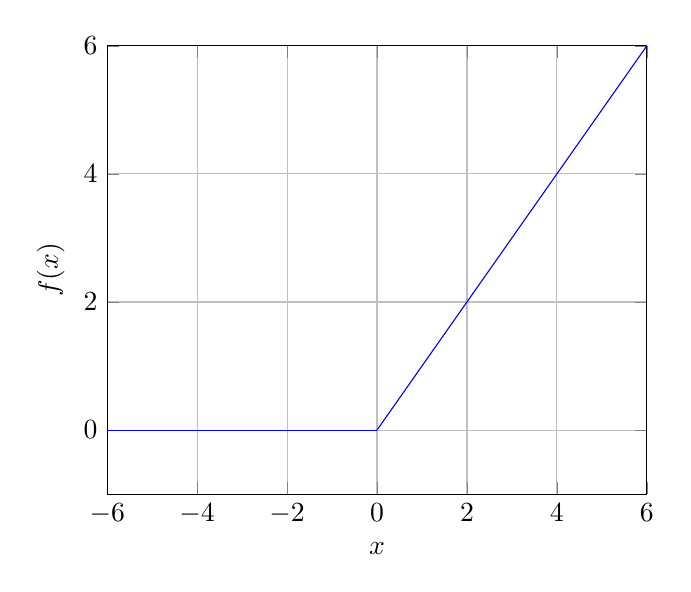
\begin{tikzpicture}
\begin{axis}[
xlabel={$x$},
ylabel={$f(x)$},
clip=false,
grid=major,
xmin=-6, xmax=6,
ymin=-1, ymax=6,
domain=-6:6
]
 \addplot+[mark=none,smooth, blue,domain=-6:0] {0};
  \addplot+[mark=none,smooth, blue,domain=0:6] {x};
\end{axis}
\end{tikzpicture}
\caption{ReLU function}
\label{fig:relu}
\end{figure}

Pooling Layer is used to perform a downsampling operation along the spatial dimensions (width, height). After all, we must reduce an input image dimensions to produce an output of expected dimensions.  It is common to periodically insert a Pooling layer in-between successive convolutional layers in a ConvNet architecture.

A simple CNN for classification could have the architecture [INPUT - CONV - RELU - POOL - FC]. For more information about CNNs, please consider the original paper\cite{krizhevsky2012imagenet}. 
